\documentclass[../../topologia_algebraica.tex]{subfiles}
\begin{document}
\section{Homotop\'ias}
\begin{defin}
  Sean $f:X\ra Y$ y $g:X\ra Y$ funciones continuas ($\star$) entre espacios topol\'ogicos $X$ y $Y$.
  Decimos que $f$ y $g$ son \emph{homot\'opicas}, denotado por $f\simeq g$, si existe una funci\'on
  continua $H:X\times[0,1]\ra Y$, que llamamos \emph{homotop\'ia}, tal que:
  \begin{itemize}
  \item Para cada par\'ametro $t\in[0,1]$, la funci\'on $H_t:X\ra Y$ definida por $H_t(x):=H(x,t)$
    es continua ($\star$).
  \item $H_0=f$ y $H_1=g$.
  \end{itemize}
  Adem\'as decimos que la \emph{homotop\'ia es relativa a} $A\subseteq X$ si para toda $x\in A$ tenemos
  que $f(x)=H_t(x)$ para toda $t\in[0,1]$, es decir la homotop\'ia fija a $A$.
\end{defin}

\begin{nota}
  La continuidad marcada por una $(\star)$ en la definici\'on anterior se puede cambiar a cualquier
  otra propiedad como ser homeomorfismos, ser morfismo de espacios basados, ser suave, etc.

  Adem\'as, de ahora en adelante denotaremos $I=[0,1]$. Antes con los lazos, esta notaci\'on pod\'ia
  confundirse en la definici\'on de homotop\'ia porque un intervalo es el dominio del lazo mientras
  que el otro intervalo parametriza la familia de lazos en la deformaci\'on.
\end{nota}

Escribimos:
\[
  \text{Map}(X,Y):=\{f:X\ra Y\mid f\;\text{es continua}\}.
\]
Si adem\'as quiero que las funciones continuas $f$ sean de espacios basados, escribo:
\[
  \text{Map}_*\Big((X,x_0),(Y,y_0)\Big):=
  \{f:(X,x_0)\ra (Y,y_o) \mid f\;\text{es continua y}\; f(x_0)=y_0\}
\]

A estos conjuntos se les puede dotar de la topolog\'ia \emph{compacto-abierto} que es la topolog\'ia
con sub-base: para todo compacto $K\subseteq X$ y todo abierto $U\subseteq Y$,
\[
  B_K(U):=\{f\in\text{Map}(X,Y) \mid f[K]\subseteq U\}.
\]


Al igual que en el caso de lazos, tenemos:

\import{\directory}{ejercicios/2} %%%%%%%%%%%%%%%%%%%%%%%%%%%%%%%%%%%%%%%%%%%%%%%%%%%%% EJERCICIO 2

Con el resultado anterior podemos definir: para dos espacios topol\'ogicos $X$ y $Y$ tenemos:
\[
  [X,Y]:=\text{Map}(X,Y)/_{\simeq}
\]
y \'este viene con un mapeo natural: $f\mapsto[f]$. La ventaja de trabajar con $[X,Y]$ y no con
$\text{Map}(X,Y)$ es que en general una funci'on continua $f:X\ra Y$ puede ser complicada de
manejar, pero en general se va a poder deformar a una funci\'on $\tilde{f}:X\ra Y$ que sea m\'as
f\'acil de manipular. Un ejemplo cl\'asico de esto es cuando una funci\'on $f$ (suave) no es transversal
a una subvariedad $Z\subset Y$ y lo deformamos para que $\tilde{f}$ s\'i sea transversal a $Z$%
%%%%%%%%%%%%%%%%%%%%%%%%%%%%%%%%%%%%%%%%%%%%%%%%%%%%%%%%%%%%%%%%%%%%%%%%%%%%%%%%%%%%%%%%%%%%% FIGURA
    \begin{figure}
      \caption{Deformaci\'on de una funci\'on $f$ para que sea transversal a $Z$ (aqu\'i est\'a
        dibujado la imagen de $f$).}
	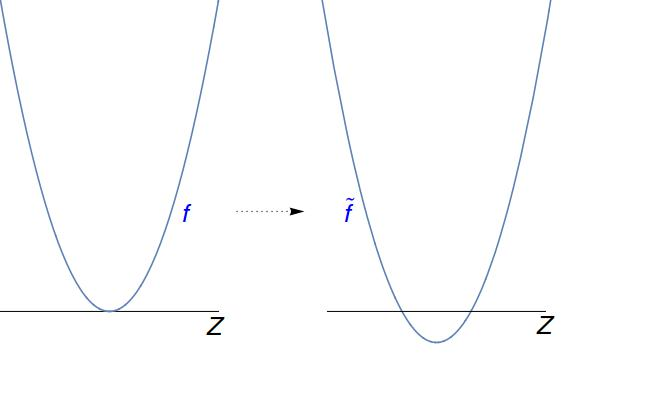
\includegraphics[scale=0.3]{transversalidad}\centering
	\label{fig:transversalidad}
      \end{figure}
%%%%%%%%%%%%%%%%%%%%%%%%%%%%%%%%%%%%%%%%%%%%%%%%%%%%%%%%%%%%%%%%%%%%%%%%%%%%%%%%%%%%%%%%%%%%%%%%%%%
(figura \ref{fig:transversalidad}).

La homotop\'ia ``preserva composiciones'':

\begin{prop}\label{prop:homotopia_composicion}
  Sean $X,Y$ y $Z$ espacios topol\'ogicos con funciones continuas $f,\tilde{f}:X\ra Y$ y
  $g,\tilde{g}:Y\ra Z$ tales que $f\simeq \tilde{f}$ y $g\simeq\tilde{g}$. Entonces
  $g\circ f\simeq \tilde{g}\circ\tilde{f}$.
\end{prop}

\begin{proof}
  Supongamos que $F:X\times I\ra Y$ y $G:Y\times I\ra Z$ son las homotop\'ias $f\simeq\tilde{f}$
  y $g\simeq\tilde{g}$ respectivamente. Definimos una funci\'on $H:X\times I\ra Z$ mediante la
  siguiente composici\'on:
  \[
    X\times I \morf{(F,\Id)} Y\times I \morf{G} Z \quad\text{con}\quad
    (x,t)\mapsto (F(x,t),t)\mapsto G(F(x,t),t). 
  \]
  $H$ es continua porque es composici\'on de funciones continuas (la primera es continua porque
  la imagen inversa de un abierto $U\times V$ de $Y\times I$ tiene como imagen inversa
  $F^{-1}[U]\times I$ que es abierto en $X\times I$ porque $F$ es continua). Ahora, para $t\in I$
  fija tenemos que $H_t=G_t(F_t(x))$ que es continua porque $F_t$ y $G_t$ lo son. Por \'ultimo
  tenemos que $H_0=G_0\circ F_0=g\circ f$ y $H_1=G_1\circ F_1=\tilde{g}\circ\tilde{f}$ por hip\'otesis.
  Concluimos que $g\circ f\simeq \tilde{g}\circ\tilde{f}$.
\end{proof}

Ahora damos un criterio importante y \'util para saber cuando dos funciones son homot\'opicos.

\begin{thm}\label{thm:homotopia_convexo}
  Sea $X$ un espacio topol\'ogico arbitrario y $Y\subseteq\RR^n$ un subespacio del espacio euclideano.
  Si $f,g:X\ra Y$ son continuas tales que para toda $x\in X$ el segmento de recta que une
  los puntos $f(x)$ y $g(x)$ en $\RR^n$, que denotamos por $\Ll_x=\overline{f(x)\, g(x)}$, est\'a
  completamente contenido en $Y$, entonces $f\simeq g$. En s\'imbolos:
  \[
    \forall x\in X, \; \Ll_x\subseteq Y \quad\then\quad f\simeq g.
  \]
\end{thm}

\begin{proof}
  Observemos que podemos parametrizar $\Ll_x$ como la trayectoria $\Ll_x(t)=(1-t)f(x)+tg(x)$ que
  empieza en el punto $f(x)$ y termina en $g(x)$. Esto nos induce un candidato a homotop\'ia:
  \[
    H:X\times I\ra Y \quad\text{con}\quad H(x,t)=\Ll_x(t)=(1-t)f(x)+tg(x).
  \]
  Observemos que por hip\'otesis $\Ll_x\subseteq Y$ entonces $H$ est\'a bien definida (ie. su
  imagen efectivamente est\'a contenido en su contradominio). S\'olo falta ver que $H$ es continua.

  Podemos descomponer la regla de correspondencia de $H$ de la siguiente manera:
  \[
    \begin{tikzcd}
      X\times I \arrow[r,"H"] \arrow[d] & Y  & (x,t) \arrow[r,mapsto,"H"] \arrow[d,mapsto]& (1-t)f(x)+tg(x) \\
      (\RR\times\RR^n)\times(\RR\times\RR^n) \arrow[r,"\cdot"] & \RR^n\times\RR^n \arrow[u,"+"']&
      (1-t,f(x),t,g(x)) \arrow[r,mapsto] & ((1-t)f(x),tg(x)) \arrow[u,mapsto]
    \end{tikzcd}
  \]
  La primera flecha hacia abajo es una funci\'on continua porque es el producto cartesiano de
  funciones continuas de variables independientes (por entrada), en particular de las cuatro funciones
  continuas $(x,t)\mapsto 1-t$, $(x,t)\mapsto f(x)$, $(x,t)\mapsto t$ y $(x,t)\mapsto g(x)$. Las
  siguientes dos flechas, correspondientes al producto por escalares y a la suma, representan
  funciones continuas (cf. ejercicio \ref{ejercicio:3}).

  Por lo tanto $H$ continua por ser composici\'on de funciones continuas. S\'olo falta verificar que:
  \[
    H_0(x)=(1-0)f(x)+0\cdot g(x)=f(x) \quad\text{y}\quad H_1(x)=(1-1)f(x)+1\cdot g(x)=g(x).
  \]
  Con esto concluimos que $H$ es una homotop\'ia entre $f$ y $g$, y que $f\simeq g$.
\end{proof}

\begin{nota}
  Observemos que si $f(x)=g(x)$, entonces $H(x,t)=(1-t)f(x)+tg(x)=f(x)-tf(x)+tf(x)=f(x)=g(x)$,
  entonces la homotop\'ia $H$ es relativo al conjunto $A=\{x\in X \mid f(x)=g(x)\}$.
\end{nota}

Los conjuntos convexos $Y\subset\RR^n$ cumplen que cualesquiera dos puntos (en particular $f(x)$ y
$g(x)$ del teorema anterior) se pueden conectar mediante un segmento de recta completamente contenido
en $Y$. Por lo tanto los conjuntos convexos cumplen de sobra las hip\'otesis del teorema anterior y
as\'i tenemos el siguiente corolario.

\begin{cor}\label{cor:homotopias_convexos}
  Si $X$ es un espacio topol\'ogico y $Y\subseteq\RR^n$ es un conjunto convexo, entonces
  $f\simeq g$ para cualesquier dos funciones continuas $f,g:X\ra Y$. En s\'imbolos:
  \[
    [X,Y]=\{e\}
  \]
  donde $e:X\ra Y$ es la funci\'on constante $e(x)=y_0$ para cualquier $y_0\in Y$.
\end{cor}

Probamos lo que nos hace falta:

\import{\directory}{ejercicios/3} %%%%%%%%%%%%%%%%%%%%%%%%%%%%%%%%%%%%%%%%%%%%%%%%%%%%% EJERCICIO 3

\end{document}